\section{Implementation of Core Functionalities}

This project contains three componets that work togather in order to makeup the entire system. In this section the inner working of each of those components will be explained.

\subsection{Lazy Koala Resource Manager (Operator)}

\ac{lazy-koala-operator} is the heart of the entire project. It is responsible for binding all other components together. In the context of Kubernetes, an operator is an agent that's running on the cluster, which is responsible for keeping one or more dedicated resources in sync with the desired state. 

For example, Kubernetes has a built-in resource named "Pod" which is the smallest deployable object in Kubernetes. So when a system administrator asked the Kube-API to create a pod out of a certain Docker container, Kube-API will create a resource object and attach it to the pod operator. Once that's done the pod operator will parse the pod resource specification and create a pod out of it. If for some reason the pod crashes or the administrator change the specification of the pod, the operator will be notified and it will re-run its reconciliation function to match the observed state with the desired state.

\begin{figure}[H]
    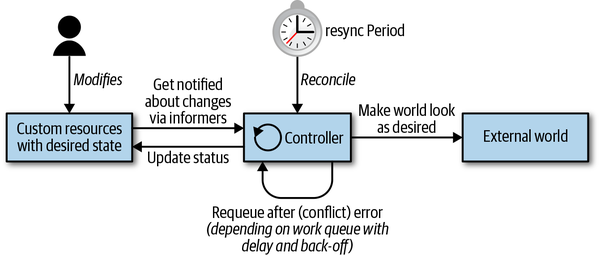
\includegraphics[width=11.5cm]{assets/implementation/kubernetes-control-loop.png}
    \caption{Kubernetes control loop \citep{hausenblas2019programming}}
    % \label{fig:reconcile-loop}
\end{figure}


Coming back to the \ac{lazy-koala-operator}, it has a Custom Resource Definition (CRD) called Inspector. In its specification, there are three required values. Deployment reference, DNS reference, and an URL to download the model that was fine-tuned for this specific deployment. So once a resource was deployed, the \ac{lazy-koala-operator} will first get the pods related to the deployment and populate the "scrapePoints" data structure with the IP address of each pod. Then it's going to find out the IP address mapped to the DNS reference and append that to the "scrapePoints". Then the \ac{lazy-koala-operator} will compare the new scrapePoints hashmap with the scrapePoints hashmap which was created in the previous iteration. Then it will identify which points needs to be added and which needs to be removed from the "gazer-config". After that the \ac{lazy-koala-operator} will pull down the "gazer-config" ConfigMap and runs the through the calculated changelog. Then it will send a patch request to the kube-api with the new state. Since this ConfigMap gets mounted to every \ac{gazer} instance via Kubernetes volumes system the changes made here will instantly be reflected with all of the \ac{gazer} instances. As a final step, an instance of \ac{sherlock} will be provisioned with the model given in the specification.

Figure \ref{fig:reconcile-loop} shows a part of this reconciliation loop, which get repeated every time there is a change to an existing resource or whenever the user creates a new variant of this resource.

\begin{figure}[H]
    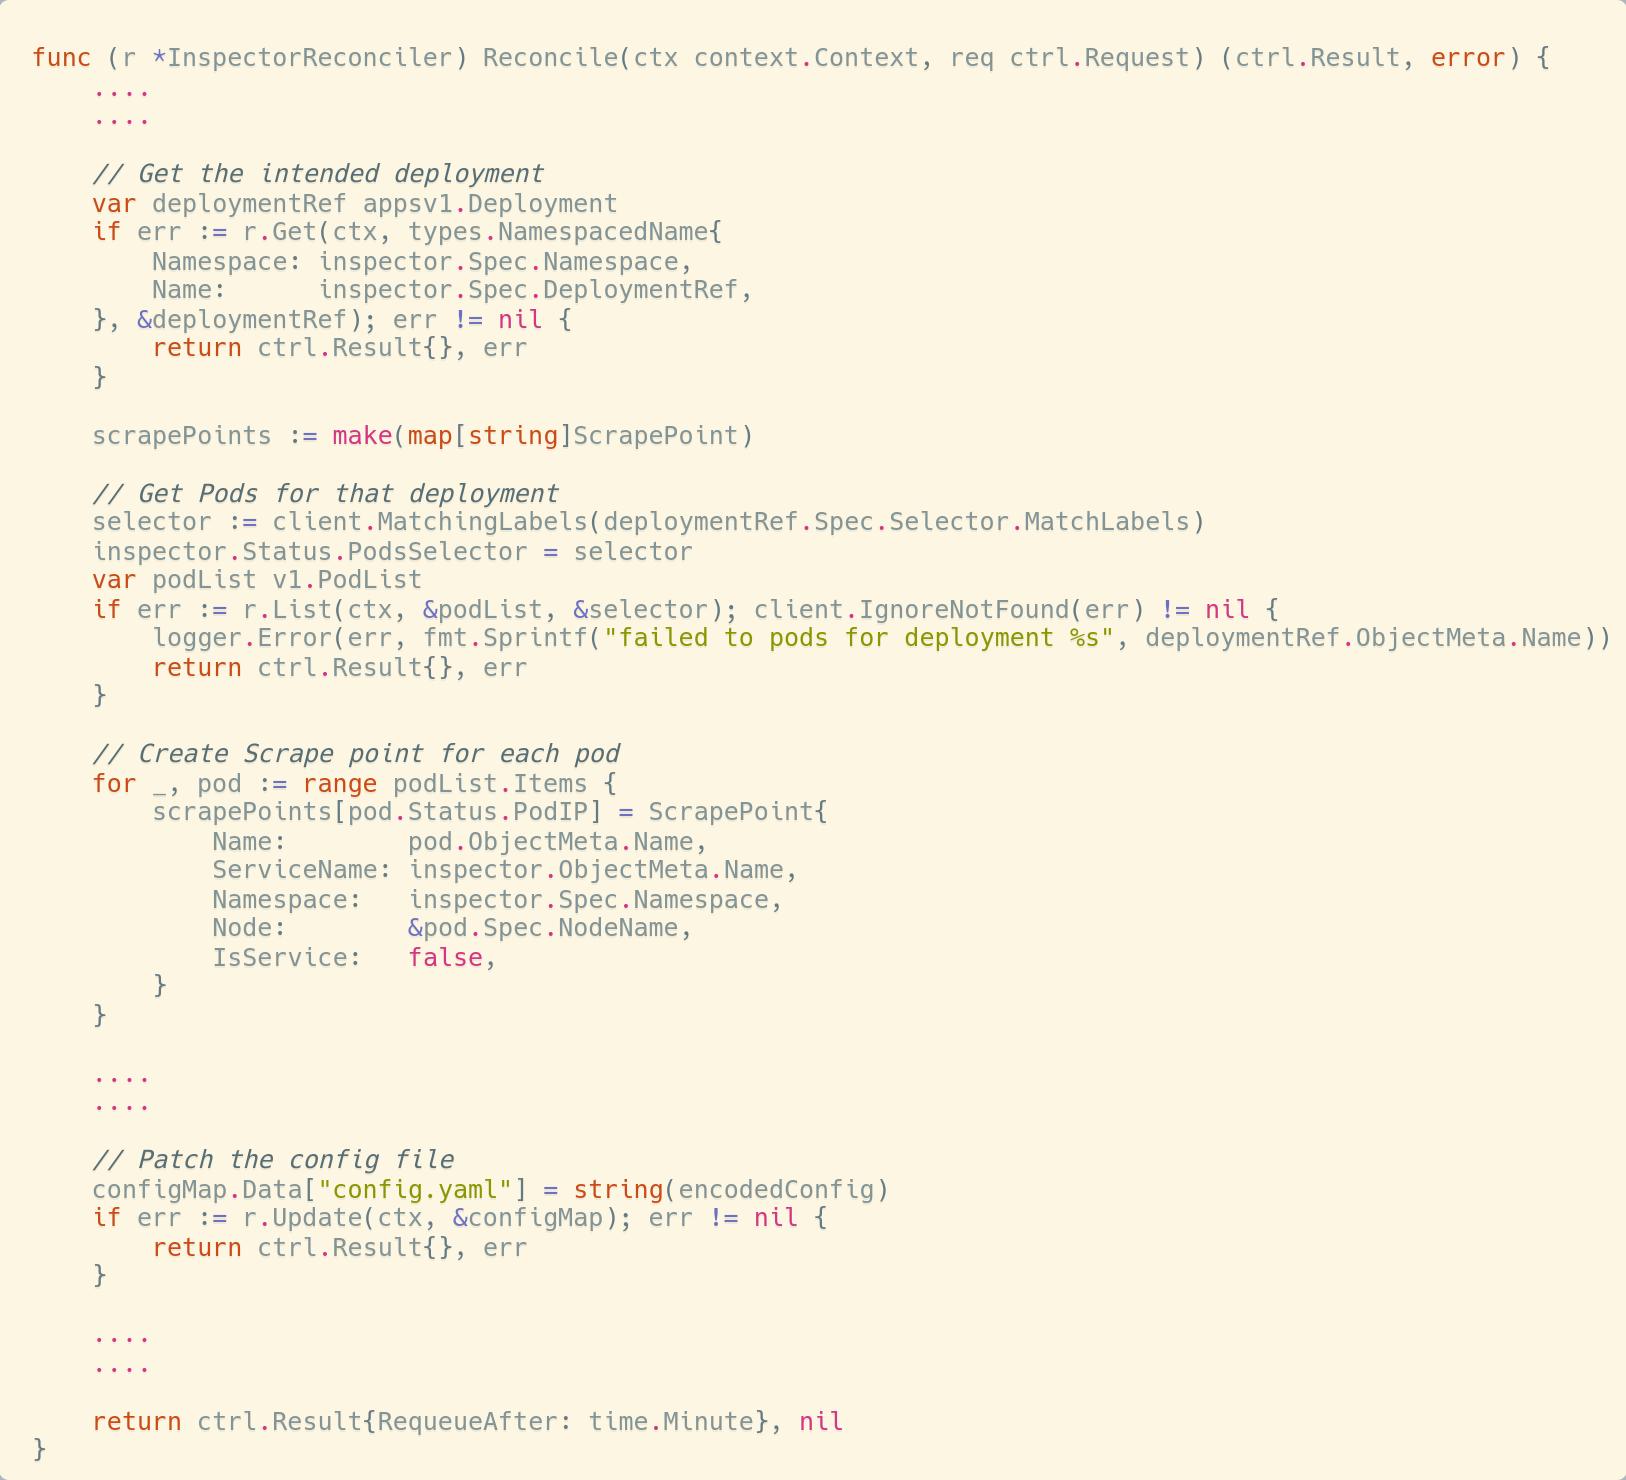
\includegraphics[height=15cm]{assets/implementation/reconcile-loop.png}
    \caption{\ac{lazy-koala-operator} reconciliation loop (self-composed)}
    \label{fig:reconcile-loop}
\end{figure}



\subsection{Telemetry extraction agent (Gazer)}

\ac{gazer} is the telemetry extraction agent that's get scheduled to run on every node on the cluster using a Kubernetes DaemonSet. \ac{gazer} is implemented in Python with the help of a library called BCC which acts as a frontend for \ac{ebpf} API. \ac{gazer} contains two kernel probes that get submitted to the kernel space at the startup. 

The first probe is a TCP SYN backlog monitor that keeps track of the backlog size of the TCP SYN queue. Every TCP connection starts with a 3-way handshake and the SYN packet is the first packet that will be sent from the client in this sequence. The entire request is kept on hold till this packet is acknowledged by the system. Hence unusually higher SYN backlog is a strong signal of something going wrong. Figure \ref{fig:backlog-probe} showcase the core part of this probe and how the backlog size is calculated.

\begin{figure}[H]
    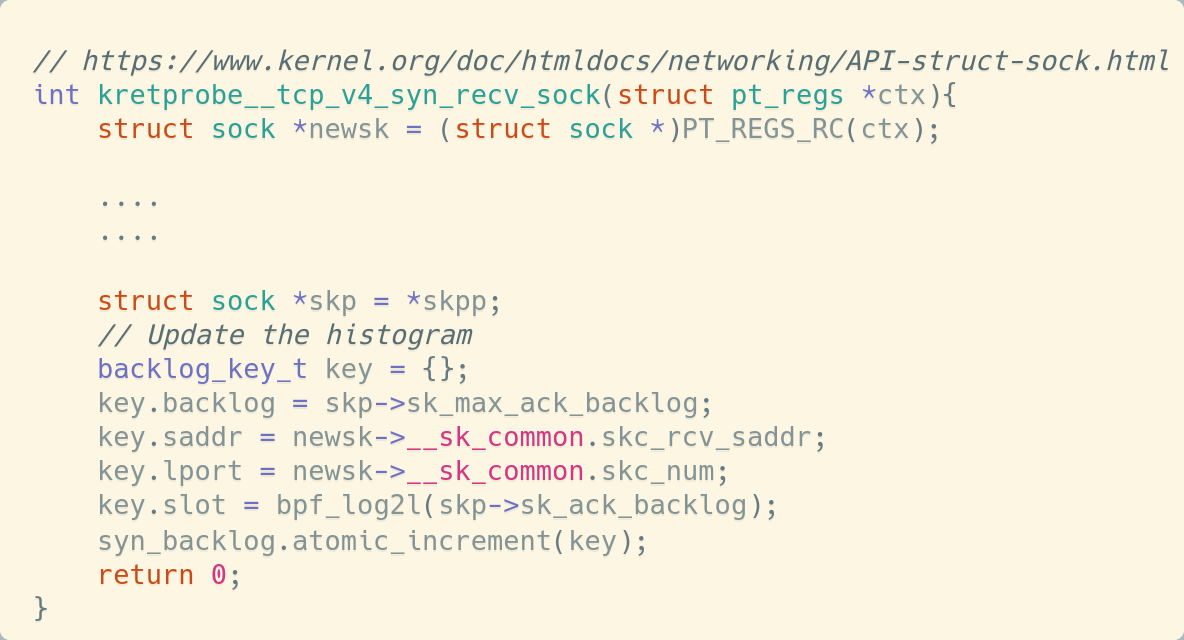
\includegraphics[width=14cm]{assets/implementation/backlog-probe.png}
    \caption{eBPF probe to collecting tcp backlog (self-composed)}
    \label{fig:backlog-probe}
\end{figure}

Next is a tracepoint probe that gets invoked whenever inet\_sock\_set\_state kernel function is called. This probe extract five key data points from every TCP request. Transmitting and receiving IP address, the number of bytes sent and received and finally the time taken to complete the entire request. All these data are shipped to the userspace via a perf buffer. In user space, these raw data get enriched with the data collected from kube-api. 

As shown in the figure \ref{fig:gazer-enrich}, since \ac{gazer} already has a list of interested IP addresses which is given by the \ac{lazy-koala-operator}, it first check whether the request was made from an one of those IPs(here only the transmitting IP is checked since every request get duplicate pair of entries, one for the request, one for the response and all the other attributes are shared among that pair). If it's found, the parser tries to identify the receiving IP address too. The receiving IP also has a match the request received and counter for that particular service will be increased. Then the parser moves on to record the number of bytes sent and received and the time taken to complete the request under identified service. Finally, these data points are exposed via an HTTP server so that the Prometheus scraper can read it and store it in the database so it can be consumed by \ac{sherlock}.

\begin{figure}[H]
    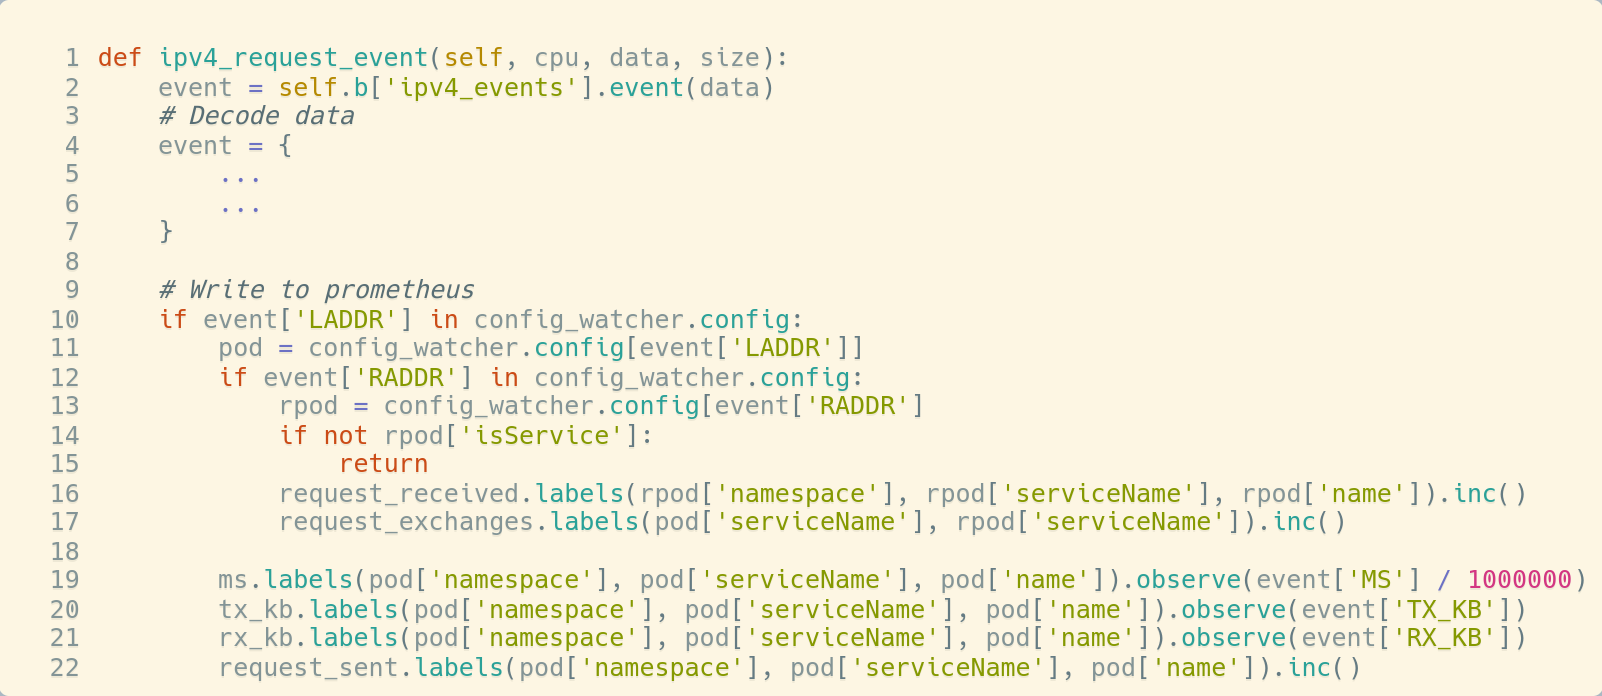
\includegraphics[width=14cm]{assets/implementation/gazer-enrich.png}
    \caption{Code used to enrich TCP event data (self-composed)}
    \label{fig:gazer-enrich}
\end{figure}


\subsection{AI-engine (Sherlock)}

\ac{sherlock} is the AI engine which predict anomaly scores for each service which in turned used by the \ac{lazy-koala-operator} to figure out possible root causes for a particular issue. From a high level, this works by polling service telemetry for a predetermined number of time steps and running it through an convolutional autoencoder which tries to reconstruct the input data sequence. The difference between the input sequence and output sequence is called the reconstruction error and this will be use as the anomaly score for this specific service. Even though this process seems straight forward, a number of prepocessing steps has to be taken in order to make it easier on the model to converge on the learning goal.

Since the collected metric data has different units, each feature of the dataset has a different range. This makes the training process very inefficient hence the model has to learn the concept of scales and unit first, and the backpropagation algorithm works best when the output values of the network are between 0-1 \citep{sola1997importance}. So to normalize this dataset a slightly modified version of the min-max normalization equation was used. This was done due to the fact that in most typical conditions metric values fluctuate between a fixed and limited range. If the min-max normalization function was applied as it is, the model may be hypersensitive to the slightest fluctuation. So adding this padding on both high and low ends, acts as an attention mechanism that helps the model to look for large variations rather than focusing on smaller ones.

\begin{figure}[H]
    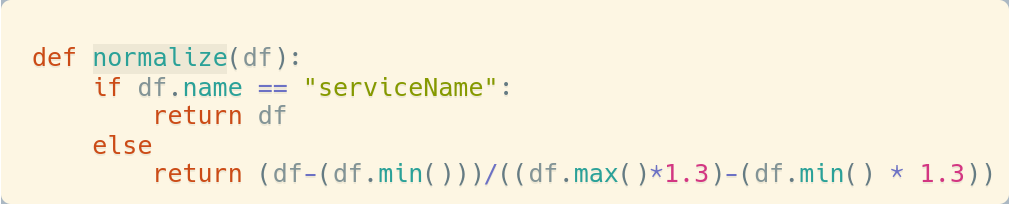
\includegraphics[width=12cm]{assets/implementation/normalize-data.png}
    \caption{Data normalization function (self-composed)}
    \label{fig:normalize-data}
\end{figure}


\begin{figure}[H]
    \centering
    \begin{subfigure}[b]{0.48\textwidth}
        \centering
        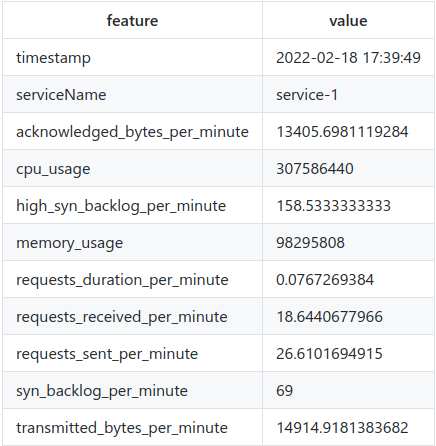
\includegraphics[width=\textwidth]{assets/implementation/before-normalization.png}
        \caption{Before Normalization}
        \label{fig:before-normalization}
    \end{subfigure}
    \hfill
    \begin{subfigure}[b]{0.49\textwidth}
        \centering
        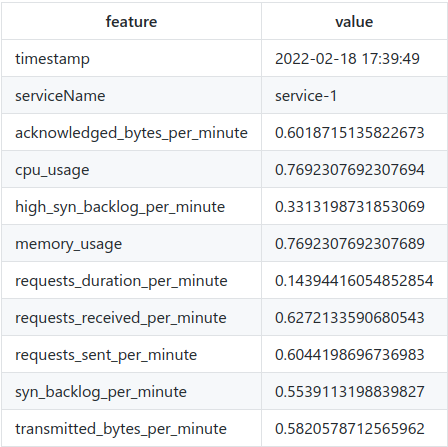
\includegraphics[width=\textwidth]{assets/implementation/after-normalization.png}
        \caption{After Normalization}
        \label{fig:after-normalization}
    \end{subfigure}
    \hfill
       \caption{Comparsion of a data point before and after the data normalization (self-composed)}
\end{figure}

% After the normalization dataset is formated to 
During the requirement engineering process it was found out even though RNN tends to perform better with time-series data, the convolutional autoencoders are very efficient at detecting anomalies from time-series data. so after the normalization step metric data is encoded into an image-like structure that can be input into a convolutional autoencoder.

\begin{figure}[H]
    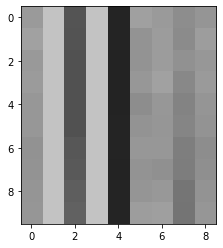
\includegraphics[height=7cm]{assets/implementation/visualize-representation.png}
    \caption{Visualization of encoded time series (self-composed)}
    \label{fig:visualize-representation}
\end{figure}